\documentclass[12pt]{article}
\usepackage[utf8]{inputenc}
\usepackage[left=1.0in,right=1.0in,top=1.0in,bottom=1.0in]{geometry}

\usepackage{amsmath}
    \usepackage{bbm}
    \usepackage{amsthm}
    \usepackage{amssymb}
    
\usepackage{tikz}
    \usepackage{pgfplots}
    \usetikzlibrary{arrows.meta}
\usepackage{float}
\usepackage{graphicx}
\usepackage{subcaption}
    
\usepackage{enumerate}
\usepackage{setspace}
\usepackage{tcolorbox}

% -------------------
% THEOREM ENVIRONMENT
% -------------------
\newtheoremstyle{break}
  {\topsep}{\topsep}% space above and below 
  {\itshape}{}      % body font
  {\bfseries}{}     %
  {\newline}{}%
\theoremstyle{break}

\newtheorem{theorem}{Theorem}[section]
\newtheorem{corollary}{Corollary}[theorem]
\newtheorem{lemma}[theorem]{Lemma}
\newtheorem{remark}[theorem]{Remark}
\newtheorem{proposition}[theorem]{Proposition}
\newtheorem{exercise}[theorem]{exercise}
\newtheorem{definition}{Definition}[theorem]
\newtheorem{example}{Example}[theorem]
% -------------------

% =========
% Commands 
% =========
\newcommand{\Prob}[1]{ 
    P\left(#1 \right) 
}
\newcommand{\Expect}[1]{
    E\left[#1 \right] 
}
\newcommand{\exponential}[1]{
    \exp\left\{#1 \right\}
}
\newcommand{\darkgreen}{blue!30!green}
\newcommand{\dgreen}{blue!30!green}
\newcommand{\lblue}{blue!50!white}



\title{High-Dimensional Probability}
\author{Jeffrey Mei}
\date{January 2019}
\onehalfspacing

\begin{document}

\maketitle

% =======================
% Chapter 1: Introduction 
% =======================


\section{Introduction}
To begin the discussion of high dimensional probability, we ought to review some basic principles of probability. Many of the results that we discuss in this course will lean heavier on moment generating functions than in introductory courses. As a consequence, we shall dive into the intuition of moment generating functions. 

Since high-dimensional probability begins with a discussion of concentration inequalities, we will also take the time to review some basic inequalities in order to make sure our tools are sharp. 
\subsection{Moment Generating Functions (MGFs)}
\begin{tcolorbox}
\begin{definition}[Moment Generating Function]
    Let $t \in \mathbb{R}.$ If it exists around the neighborhood $t=0$, we define the moment generating function of the RV $X$ as 
    \begin{equation}
    M_X(t) = E\left[e^{tX}\right] 
    \end{equation}
\end{definition}
\end{tcolorbox}


Moment generating functions are important theoretical objects in probability theory. Primarily, they are important because they can uniquely characterize a probability distribution and allow us to easily obtain the $n$th moment of any distribution. In a sense, they capture the "soul" of a probability distribution. To understand the underlying mathematical machinery of moment generating functions further, notice that the MGFs can be represented as follows:

% Equation
\begin{align*}
    M(t) &= E[ e^{tX} ]     \\ 
    &= E\left[ 1 + tX + \frac{t^2 X^2}{2!} + ... + \frac{t^n X^n}{n!} + ...\right] && \text{series expansion}\\
    &= E\left[ 1 \right] + E\left[tX\right] + E\left[\frac{t^2 X^2}{2!}\right] + ... + E\left[\frac{t^n X^n}{n!}\right]+... &&\text{property of expectation} \\
    &= 1 + tE[X] + \frac{t^2}{2!}E[X^2] + ... + \frac{t^n}{n!} E[X^n] + ...
\end{align*}

\noindent Now, with the expanded form of the MGF, we can easily obtain the $n$th moment of the random variable $X$. The following box summarizes this procedure succintly, and Figure \ref{fig:MGF} illustrates the intuition. \\

\begin{tcolorbox}[colback=white!90!gray, title=Intuition: Find the $n$th moment of $X$]
\begin{enumerate}
    \item expand series $E[e^{tX}]$
    \item take the $n$th derivative
    \begin{itemize}
        \item the first $(n-1)$ terms go to 0 
    \end{itemize}
    \item set $t=0$
    \begin{itemize}
        \item terms $(n+1), (n+2), ...$ go to 0
    \end{itemize}
\end{enumerate}
\end{tcolorbox}

% Illustration of MGF
\begin{figure}[H]
\centering
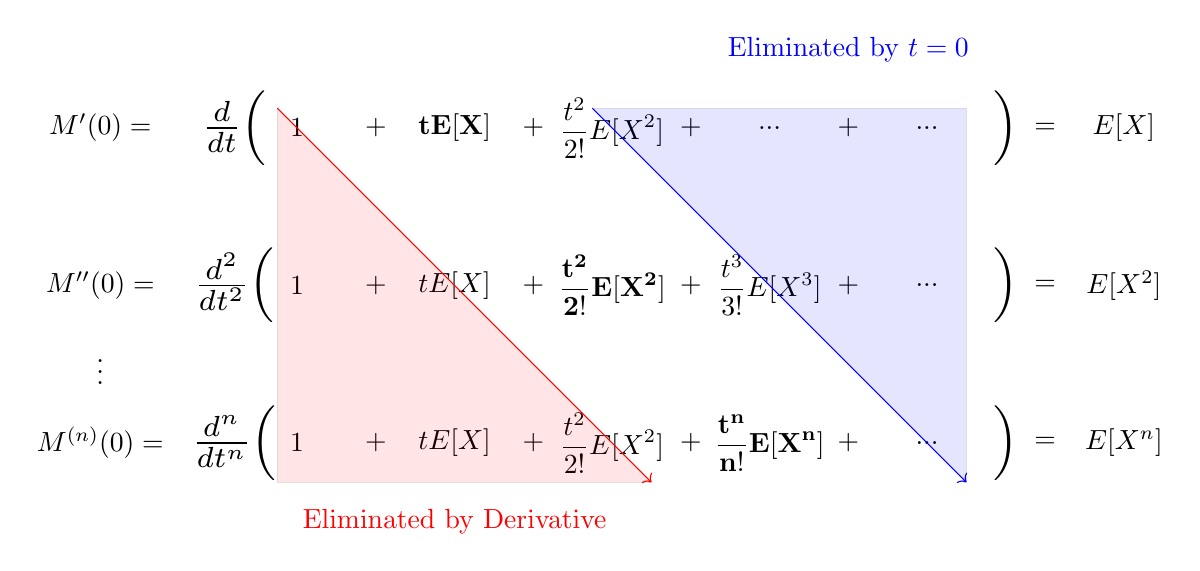
\begin{tikzpicture}

    % 1st Row 
    % -------
    \node[] (10) at (0,0) {1};        
    \node[] (11) at (2,0) {$\mathbf{\displaystyle{tE[X]}}$};  
    \node[] (12) at (4,0) {$\displaystyle{\frac{t^2}{2!}E[X^2]}$}; 
    \node[] (1k) at (6,0) {$...$}; 
    \node[] (1n) at (8,0) {$...$}; 
    \node[] (1n) at (10.5,0) {$E[X]$}; 
    
    \node[] at (1,0) {$+$};
    \node[] at (3,0) {$+$};
    \node[] at (5,0) {$+$};
    \node[] at (7,0) {$+$};
    \node[] at (9.5,0) {$=$};
    
    % 2nd Row 
    % -------
    \node[] (20) at (0,-2) {1};        
    \node[] (21) at (2,-2) {$\displaystyle{tE[X]}$};  
    \node[] (22) at (4,-2) {$\mathbf{\displaystyle{\frac{t^2}{2!}E[X^2]}}$}; 
    \node[] (2k) at (6,-2) {$\displaystyle{\frac{t^3}{3!}E[X^3]}$}; 
    \node[] (2n) at (8,-2) {$...$}; 
    \node[] (1n) at (10.5,-2) {$E[X^2]$}; 
    
    \node[] at (1,-2) {$+$};
    \node[] at (3,-2) {$+$};
    \node[] at (5,-2) {$+$};
    \node[] at (7,-2) {$+$};
    \node[] at (9.5,-2) {$=$};
    
    % 3rd Row 
    % -------
    \node[] (30) at (0,-4) {1};        
    \node[] (31) at (2,-4) {$\displaystyle{tE[X]}$};  
    \node[] (32) at (4,-4) {$\displaystyle{\frac{t^2}{2!}E[X^2]}$}; 
    \node[] (3n) at (6,-4) {$\mathbf{\displaystyle{\frac{t^n}{n!}E[X^n]}}$}; 
    \node[] (3k) at (8,-4) {$...$}; 
    \node[] (1n) at (10.5,-4) {$E[X^n]$}; 
    
    \node[] at (1,-4) {$+$};
    \node[] at (3,-4) {$+$};
    \node[] at (5,-4) {$+$};
    \node[] at (7,-4) {$+$};
    \node[] at (9.5,-4) {$=$};
    
    % Draw Paths 
    % ----------
    \draw[red , ->] (-0.25,0.25) -- ( 4.5,-4.5);
    \draw[blue, ->] ( 3.75,0.25) -- ( 8.5,-4.5);
    \draw[fill=red,opacity=0.1] (-0.25,0.25) -- (-0.25,-4.5) -- (4.5,-4.5);
    \draw[fill=blue,opacity=0.1] ( 3.75,0.25) -- ( 8.5,0.25) -- (8.5,-4.5);
    
    % Labels
    % ------
    \node[red]  at (2,-5) {Eliminated by Derivative};
    \node[blue] at (7, 1) {Eliminated by $t=0$};
    \node[] at (-2.5, 0) {$M'(0)=$};
    \node[] at (-2.5,-2) {$M''(0)=$};
    \node[] at (-2.5,-3) {$\vdots$};
    \node[] at (-2.5,-4) {$M^{(n)}(0)=$};
    
    \node[scale=1.5] at (-0.8, 0) {$\frac{d}{dt}\Big($}; 
    \node[scale=1.5] at (-0.8,-2) {$\frac{d^2}{dt^2}\Big($}; 
    \node[scale=1.5] at (-0.8,-4) {$\frac{d^n}{dt^n}\Big($}; 
    \node[scale=1.5] at (9, 0) {$\Big)$}; 
    \node[scale=1.5] at (9,-2) {$\Big)$}; 
    \node[scale=1.5] at (9,-4) {$\Big)$}; 
    
\end{tikzpicture}
\label{fig:MGF}
\caption{Illustration of Obtaining $n$th Moment of $X$}
\end{figure}



\subsection{Classical Inequalities}
The purpose of this section is to review and continue developing tools and techniques that we can apply to later proofs.  

% ========================
% Lemma: Integral Identity
% ========================
\begin{tcolorbox}
\begin{lemma}[Integral Identity]
Suppose $X$ is a non-negative RV. It follows that 
    \begin{equation}
    E[X] = \int_{0}^{\infty}P(X > t)dt
    \end{equation}
\end{lemma}
\end{tcolorbox}

\begin{proof}
    Suppose $x \geq 0$ is a non-negative real-valued number. It follows that 
    
    \begin{align*}
        x &= \int_{0}^{x} 1 dt = \int_{0}^{\infty} \mathbbm{1}\{x > t\}dt. 
    \end{align*}
    
    Since the above equality holds for any $x \in \mathbb{R} \geq 0$, the equality holds for any random variable $X$ that is non-negative and real-valued. Therefore, by substituting $X$ for $x$ and taking the expectation of both sides, we obtain 
    
    \begin{align*}
        X &= \int_{0}^{X} 1 dt = \int_{0}^{\infty} \mathbbm{1}\{X > t\}dt && \\
        \implies E[X] &= E\left[\int_{0}^{\infty} \mathbbm{1}\{X > t\}dt\right] && \\ 
        &= \int_{0}^{\infty} E\left[\mathbbm{1}\{X > t\}\right]dt &&\text{Fubini-Tonelli} \\
        &= \int_{0}^{\infty} P(X > t) dt && \\ 
    \end{align*}
\end{proof}

\begin{tcolorbox}
\begin{lemma}[Integral Identity (Extension)]
Suppose $X$ is a RV. It follows that 
    \begin{equation}
    E[X] = \int_{0}^{\infty}P(X>t)dt - \int_{-\infty}^{0}P(X < t)dt.
    \end{equation}
\end{lemma}
\end{tcolorbox}

\begin{proof}
Suppose $x\in \mathbb{R}$. We observe that 
    \[ x = 
    \begin{cases}
        \displaystyle{-\int_{-\infty}^{0} \mathbbm{1}\{t > x\} dt} &, x < 0 \\
        \displaystyle{\int_{0}^{\infty} \mathbbm{1}\{t < x\} dt} &, x \geq 0 
    \end{cases}
    \] 
Furthermore, since one of the integrals will be 0, we have  
    \begin{align*}
    x &= \int_{0}^{\infty} \mathbbm{1}\{x>t\}dt - \int_{-\infty}^{0}\mathbbm{1}\{x<t\}dt \\
    X &= \int_{0}^{\infty} \mathbbm{1}\{X>t\}dt - \int_{-\infty}^{0}\mathbbm{1}\{X<t\}dt && \text{Allow $x$ to be a RV}\\
    \implies E[X] &= E\left[\int_{0}^{\infty} \mathbbm{1}\{X>t\}dt\right] - E\left[\int_{-\infty}^{0}\mathbbm{1}\{X<t\}dt\right] && \text{Take expectation}\\
    E[X] &= \int_{0}^{\infty} E\left[\mathbbm{1}\{X>t\}dt\right] - \int_{-\infty}^{0}E\left[\mathbbm{1}\{X<t\}dt\right] && \text{Fubini-Tonelli}\\
    &= \int_{0}^{\infty} P(X > t)dt - \int_{-\infty}^{0}P(X<t)dt 
    \end{align*}
\end{proof}

% ================================
% Proposition: Markov's Inequality
% ================================
\begin{tcolorbox}
\begin{proposition}[Markov's Inequality]
For any non-negative RV, $X$, and $t>0$, 
    \begin{equation}
    P(X \geq t) \leq \frac{E[X]}{t}
    \end{equation}
\end{proposition}
\end{tcolorbox}

\begin{proof}
\begin{align*}
    E[X] &= \int_{0}^{\infty} xp(x)dx && \text{defn. of expectation} \\ 
    &= \int_{0}^{t} xp(x)dx + \int_{t}^{\infty}xp(x)dx && \text{separate integral} \\
    \implies E[X] &\geq \qquad \qquad \qquad \int_{t}^{\infty}xp(x)dx && \text{since $\int_{0}^{t}xp(x)dx \geq 0$} \\
    &\geq \qquad \qquad \qquad \int_{t}^{\infty} tp(x)dx &&\text{since $x \geq t$ in the integral} \\ 
    &= \qquad \qquad \qquad t \int_{t}^{\infty}p(x)dx && \text{since we're not integrating over $t$} \\ 
    &= \qquad \qquad \qquad t P(X \geq t)  \\
    \implies P(X \geq t) &\leq \frac{E[X]}{t}
\end{align*}
\end{proof}


% ===================================
% Proposition: Chebyshev's Inequality
% ===================================
\begin{tcolorbox}
\begin{proposition}[Chebyshev's Inequality]
Suppose $X$ has a finite mean and variance. It follows that 
    \begin{equation}
    P(|X-\mu| \geq t) \leq \frac{\sigma^2}{t^2}
    \end{equation}
\end{proposition}
\end{tcolorbox}

\begin{figure}[H]
    \centering
    \includegraphics[scale=0.7]{Chebyshev.png}
    \caption{Simulations for Chebyshev's Inequality. We see that the Chebyshev inequality is actually conservative for small $t$, but becomes better as $t$ increases. }
    \label{fig:chebyshev_sim}
\end{figure}
\begin{figure}[H]
    \centering
    \includegraphics[scale=0.7]{Markov.png}
    \caption{Simulations for Markov's Inequality. Similar to Chebyshev's inequality, the inequality improves for larger $t$. However, the simulated value is constant.}
    \label{fig:markov_sim}
\end{figure}




% =====================================
% Chapter 2: Concentration Inequalities
% =====================================
\pagebreak
\section{Concentration Inequalities}

The topic of concentration inequalities is a collection of methods and techniques that are used to quantify how much a random variable deviates from its mean. The simplest and most well-known concentration inequality is Chebyshev's inequality -- relating deviations from the mean with the variance of the random variable. Other examples of concentration inequality results include the law of large numbers (because it is a direct result of Chebyshev's inequality), describing the deviation of the sample mean from the true mean. 

Concentration inequalities are powerful and have become a topic of recent interest because it resolves some issues left from classical statistics. Classical results include the law of large numbers and central limit theorem. Although these results are widespread and are powerful in their own right, they are largely qualitative results. 

\indent  - The LLN simply states that the sample mean converges (in probability) towards the true mean of a random variable, but fails to state how quickly the sample mean converges. 

\indent - The CLT simply states that the distribution of the sample mean converges towards the normal distribution for large sample sizes, but fails to state how quickly the distribution converges.  

Whereas classical results \textit{qualitatively} describe convergence behavior, concentration inequalities promise to \textit{quantitatively} describe convergence behavior. This is of particular interest in the age of big data. As statistics transitioned from an esoteric mathematical world into a data-filled modern world, we could no longer fall back on classical methods and relegate sample sizes to infinity. We had to create new methods that were more tangible and could handle concrete sample sizes. 

The recent interest in concentration inequalities has not only improved classical results, but has also been of interest to the rising field of machine learning. Concentration inequalities play a role in learning algorithms because they quantify an algorithm's learning rate. 

In this section, we will introduce several methods for quantifying closeness to the mean in terms of sample size, obtaining tighter bounds, as well as illustrate various qualitative properties we hope to achieve while developing concentration inequalities.  


% \begin{example}[Chebyshev's Inequality]
% \begin{align*}
%     P\left(S_n \geq \frac{3}{4}N\right) &= P\left(S_n - \frac{N}{2} \geq \frac{N}{4} \right) \\
%     &\leq P\left(S_n - \frac{N}{2} \geq \frac{N}{4} \right) + P\left( S_n - \frac{N}{2} \leq -\frac{N}{4}\right) && \text{since $0 \leq P(E)$} \\ 
%     &= P\left(\left|S_n - \frac{N}{2}\right| \geq \frac{N}{4} \right) && \text{defn. of abs. val.} \\
%     &\leq \frac{(N/4)}{(N/4)^2} && \text{Chebyshev's Inequality} \\ 
%     &= \frac{4}{N}
% \end{align*}    
% \end{example}



% Hoeffding's Inequality for Symmetric Bernoulli
\subsection{Hoeffding's Inequality}
To begin, we will consider one of the simplest concentration inequalities, while demonstrating a powerful technique for finding a concentration inequality. The Hoeffding's inequality that we will consider only considers symmetric Bernoulli random variables. The technique will bind the moment generating function. 



% ==================================
% Definition: Symmetric Bernoulli RV
% ==================================
\begin{tcolorbox}
\begin{definition}[Symmetric Bernoulli Random Variables]
A random variable is said to have a symmetric Bernoulli distribution (also known as Rademacher distribution) if 
$$P(X=-1) = P(X=1) = 1/2.$$
\end{definition}
\begin{remark}
Alternatively, the distribution may be constructed from the Bernoulli distribution. Suppose $X \sim Bernoulli(1/2)$ and define $Y = 2X-1$. It follows that $Y$ follows the symmetric Bernoulli distribution. 
\end{remark}
\end{tcolorbox}

% ===============================
% Theorem: Hoeffding's Inequality
% ===============================
\begin{tcolorbox}
\begin{theorem}[Hoeffding's Inequality]
    Assumptions:
    \begin{itemize}
    \item $X_1, ..., X_n$ independent and Symmetric Bernoulli RVs
    \item $a = (a_1, ..., a_N) \in \mathbb{R}^N$
    \item $t \geq 0$
    \end{itemize}
    \begin{equation}
        \implies P\left(\sum_{i=1}^{N} a_i X_i \geq t\right) \leq \exp{\left(-\frac{t^2}{2\|a\|_{2}^{2}}\right)}
    \end{equation}
    In particular, for the sample mean such that $a_i = 1/N$ for $i=1,...,N$, 
    \begin{equation}
        P\left(\frac{1}{N}\sum_{i=1}^{N} X_i \geq t\right) \leq \exp{\left(-\frac{t^2}{2}\right)}
    \end{equation}
\end{theorem}
\end{tcolorbox}

% Proof 
\begin{proof}
    \begin{align*}
        P\left( \sum_{i=1}^{N} a_i X_i > t \right) &= P\left( \lambda\sum_{i=1}^{N} a_i X_i > \lambda t \right) && \text{we will optimize for $\lambda$ later} \\
        &= P\left( \exp\left(\lambda\sum_{i=1}^{N} a_i X_i\right) > \exp\left(\lambda t\right) \right) && \text{exponentiate both sides} \\
        &\leq \frac{ E\left[ \exp\left(\lambda\sum_{i=1}^{N} a_i X_i\right) \right] }{\exp(\lambda t)} && \text{Markov's Inequality} \\ 
        &= \exp(-\lambda t) E\left[ \prod_{i=1}^{N}e^{\lambda a_i X_i} \right] \\ 
        &= \exp(-\lambda t) \prod_{i=1}^{N} E\left[ e^{\lambda a_i X_i} \right] && \text{b/c iid} \\ 
        &= \exp(-\lambda t) \prod_{i=1}^{N} M_{X_i}(\lambda a_i) && \text{Defn. of MGF} \\ 
    \end{align*}
    Consider an individual $i$. It follows that 
    \begin{align*}
        M_{X_i} &= E\left[ e^{\lambda a_i X_i} \right] && \text{defn. of MGF} \\ 
        &= \frac{1}{2} e^{\lambda a_i} + \frac{1}{2} e^{-\lambda a_i} && \text{since $X_i \in \{-1,1\}$} \\ 
        &= \frac{e^{\lambda a_i} + e^{-\lambda a_i}}{2} \\ 
        &= \cosh( \lambda a_i ). 
    \end{align*}
    We will also make the following observation:
    \begin{align*}
        \cosh(x) \leq e^{x^2/2}. \\ 
    \end{align*}
    We can see that this is true using the Taylor expansion of both sides, comparing $e^{x^2/2}$ with $\cosh(x)$ to obtain 
    \begin{align*}
        e^{x^2/2} &= 1 &&+ \frac{x^2}{(2)(1!)} &&&+ \frac{x^4}{(4)(2!)} &&&&+ \frac{x^6}{(8)(3!)} &&&&&+ ... \\ 
        \cosh(x) &= 1 &&+ \frac{x^2}{2!} &&&+ \frac{x^4}{4!} &&&&+ \frac{x^6}{6!} &&&&&+ ... \\ 
    \end{align*}
    It is easy to see that through the Taylor expansion of both $\cosh(x)$ and $e^{x^2/2}$, $\cosh(x) \leq e^{x^2/2}.$
    
    
    \noindent Returning back to the proof, we have 
    \begin{align*}
        P\left( \sum_{i=1}^{N} a_i X_i > t \right) 
            &\leq \exp(-\lambda t) \prod_{i=1}^{N} M_{X_i}(\lambda a_i) \\ 
        &\leq \exp(-\lambda t) \prod_{i=1}^{N} e^{\lambda^2 a_i^2 /2} && \text{since $M_{X_i} = \cosh(x) \leq e^{x^2/2}$} \\
        &= \exp\left( \frac{\lambda^2}{2} \sum_{i=1}^{N}a_i^2 - \lambda t \right) \\ 
        &= \exp\left( \frac{\lambda^2}{2} - \lambda t \right) && \text{since $||a||_2=1$ } 
    \end{align*}
    Now, we see that in order to get a tight upper bound, we must minimize $\exp(\lambda^2/2 - \lambda t).$ By setting $\lambda=t$, we obtain
    \begin{align*}
        P\left(\sum_{i=1}^{N} a_i X_i > t \right) &\leq \exp \left( t^2/2 - t^2 \right) \\
        &= e^{-t^2/2}
    \end{align*}
\end{proof}

\begin{tcolorbox}[colback=white!90!gray, title=Proof Technique: Hoeffding's Inequality]
\begin{enumerate}
    \item multiply both sides by $\lambda$ (in order to have an optimizing constant)
    \item exponentiate both sides (in order to get MGF)
    \item apply Markov's inequality 
    \item bind MGF with some exponential tail 
    \item optimize in $\lambda$ to find tight final upper bound
\end{enumerate}
\end{tcolorbox}


\begin{tcolorbox}
\begin{theorem}[Hoeffding's Inequality for Bounded Random Variables]
Let $X_1, ..., X_N$ be independent random variables within the bounds $[m_i, M_i]$. It follows for $t > 0$ that 
    \begin{equation}
    \Prob{\sum_{i=1}^{N} (X_i - E[X_i]) \geq t} \leq \exponential{-\frac{2t^2}{\sum_{i=1}^{N}(M_i - m_i)^2}} \\ 
    \end{equation}
\end{theorem}
\end{tcolorbox}

% =============
% Generalized Hoeffding
% =============
\begin{proof}
    Following a similar proof structure for the Hoeffding's inequality, we will bind the moment generating function.  
    \begin{align*}
    \Prob{\sum_{i=1}^{N}(X_i - E[X_i]) \geq t} &= \Prob{ \exponential{ \lambda\sum_{i=1}^{N}( X_i - E[X_i])} \geq \exponential{\lambda t}} && 
        \text{}  \\
    &\leq \frac{ \Expect{ \exponential{\lambda \sum_{i=1}^{N} (X_i - \mu_i )} } }{ \exponential{\lambda t} } && \text{Markov Inequality} \\ 
    &= \frac{ \prod_{i=1}^{N} \Expect{\exponential{\lambda(X_i - \mu_i)}} }{\exponential{\lambda t}} && 
        \text{} \\
    \end{align*}
    % 
    Consider an individual $i$. For probability distribution $f(x),$ it follows that 
    % 
    \begin{align*}
    \Expect{\exponential{\lambda(X_i - \mu_i)}} = \int_{m_i}^{M_i} e^{\lambda(x - \mu_i)}f(x) dx
    \end{align*}
    Notice that $f(x) \leq \textcolor{red}{???}$ for bounded random variables, then we can create an exponential bound on $\Expect{\exponential{\lambda(X_i - \mu_i)}}$. From here, we can easily create the bound 
\end{proof}
% =============

\begin{tcolorbox}
    \begin{example}[Boosting Randomized Algorithms]
    In machine learning, we often need to classify objects into corresponding categories (e.g. provided an image, is it a picture of a cat or a dog?). Boosting is a technique that employs several algorithms to individually categorize objects. However, the algorithms may not always agree. Therefore, the final decision is determined by a majority vote on the classification of the observation. Let us now consider a randomized algorithm. 
    
    Suppose an algorithm has a chance of making the correct decision with probability $1/2 + \delta$ for $\delta>0$. We will boost this algorithm by running the algorithm $N$ times, and then finalizing our decision with a majority vote. Show that for $\varepsilon \in (0,1),$ the answer is correct with probability $1-\varepsilon$ as long as 
    $$ N \geq \frac{\ln{(1/\varepsilon)}}{2\delta^2} $$
    \end{example}
\end{tcolorbox}
\begin{proof}
    To begin, let us define some variables. 
    \begin{align*}
    & \cdot X_i \sim Bernoulli(1/2 + \delta) \\ 
    & \cdot X_i = 1 && i\text{th algorithm makes incorrect decision} \\ 
    & \cdot X_i = 0 && i\text{th algorithm makes correct decision} \\ 
    & \cdot P(X_i = 1) = 1/2 - \delta && \text{P(Incorrect Decision)} \\ 
    & \cdot P(X_i = 0) = 1/2 + \delta && \text{P(Correct Decision)} \\ 
    & \cdot S_n = \sum_{i=1}^{N}X_i && \text{Number of Incorrect Decisions} \\ 
    \end{align*}
    
    \begin{align*}
    \Prob{\sum_{i=1}^{N}\left(X_i - \Expect{X_i}\right) \geq t} &\leq \exponential{-\frac{2t^2}{\sum_{i=1}^{N}\left(M_i - m_i\right)^2}} && \text{Hoeffding's Inequality} \\ 
    % 
    \implies \Prob{\sum_{i=1}^{N}\left(X_i - \textcolor{\darkgreen}{ \left(\frac{1}{2} - \delta \right)}\right) \geq t} &\leq \exponential{-\frac{2t^2}{\sum_{i=1}^{N}\left(\textcolor{\darkgreen}{1 - 0}\right)^2}} && \text{$E[X_i] = \frac{1}{2} - \delta; M_i = 1; m_i = 0$} \\ 
    &= \exponential{-\frac{2t^2}{\textcolor{\darkgreen}{N}}} 
    \end{align*}
%    Our goal is to get the right hand exponential tail be the error term $\varepsilon$. This means that the centered $X_i$ must exceed $(1/2 + \delta)$ in order to result in an incorrect decision within the $i$th iteration of the boosting algorithm. Therefore, we shall let $t = 1/2 + \delta$. It follows that 
% \begin{align*}
% \Prob{\sum_{i=1}^{N}\left( X_i - \left(\frac{1}{2} - \delta\right) \geq \frac{1}{2} + \delta \right)}  &\leq \exponential{-\frac{2\textcolor{\darkgreen}{(1/2+\delta)^2}}{N}} &&  
%     \text{ Let $t = 1/2 + \delta$ }  \\
% &= \exponential{-\frac{2(\textcolor{\darkgreen}{1/4 + \delta + \delta^2)}}{N}} && \text{} \\
% &\leq \exponential{
%     -\left(\frac{1}{2N} \right)
% } = \varepsilon 
% \end{align*}
% Let us now consider the value of $N$ needed in order for the above expression to hold. 
% \begin{align*}
% \exponential{
%     -\left(\frac{1}{2N} \right)
% } &= \varepsilon \\ 
% \left(\frac{1}{2N} \right) &= -\ln{\varepsilon} && \text{take log of both sides} \\
% &= \ln(1/\varepsilon) \\ 
% \end{align*}
    Let $t = \delta/2$ because \textcolor{red}{??????} because it works.
    It follows that we have
    \begin{align*}
    \varepsilon = \exponential{-\frac{2t^2}{N}} &= \exponential{-\frac{2\textcolor{\darkgreen}{\delta^2}}{\textcolor{\darkgreen}{4 }N}} && 
        \text{assign $\varepsilon$} \\ 
    &= \exponential{-\frac{\delta^2}{2 N}} && 
        \text{} \\ 
    -\ln(\varepsilon)  &= \frac{\delta^2}{2 N} \\ 
    N &= -\frac{1}{\ln{(\varepsilon)}2\delta^2} \\ 
    &= \frac{1}{\ln{(1/\varepsilon)} 2\delta^2} 
    \end{align*}
\end{proof}




\subsection{Chernoff Bounds}
The method to derive Chernoff bounds is nearly identical to the method used to derive Hoeffding's inequality. The sole difference is that the MGF is bounded by the inequality $1+x \leq e^x$ instead of $\frac{e^x + e^{-x}}{2} \leq e^{x^2/2}.$ \\ 

\begin{tcolorbox}
\begin{theorem}[Chernoff Inequality]
Suppose $X1, .., X_N$ are independent Bernoulli random variables with probabilities $p_1, ..., p_N$ with $S_N = \sum_{i=1}^{N}X_i$ and $E[S_N] = \mu$, then
    \begin{equation}
    P(S_n \geq t) \leq e^{-\mu}\left(\frac{e \mu}{t}\right)^t
    \label{eq:chernoff1}
    \end{equation}
Alternatively, for $\delta \in (0,1],$ the Chernoff Inequality may be written as 
    \begin{equation}
    P\left(|S_n-\mu| \geq \delta \mu \right) \leq 2e^{-c \mu \delta^2}
    \label{eq:chernoff2}
    \end{equation}
\label{theorem:chernoff}
\end{theorem}
\end{tcolorbox}

\begin{proof}
\begin{align*}
    P(S_n \geq t) &= P\left(\sum_{i=1}^{N}X_i \geq t\right) \\
    &= P\left(\lambda\sum_{i=1}^{N}X_i \geq \lambda t\right) &&\text{multiply both sides by $\lambda$} \\
    &= P\left( \exp\left\{\lambda\sum_{i=1}^{N}X_i\right\} \geq 
        \exp\left\{\lambda t \right\} \right) && \text{exponentiate both sides} \\
    &\leq \frac{E\left[\exp\left\{\lambda \sum_{i=1}^{N}X_i \right\}\right]}{\exp\left\{ \lambda t \right\}} &&\text{Apply Markov's inequality} \\ 
    &\leq \frac{\prod_{i=1}^{N} E\left[\exp\left\{\lambda X_i \right\}\right]}{\exp\left\{ \lambda t \right\}} &&\text{} \\ 
\end{align*}

For a single RV $X_i$, we have 
\begin{align*}
E\left[e^{\lambda X_i}\right] &= (1-p_i) e^{(\lambda)(0)} + p_i e^{ (\lambda)(1) } &&\text{Expectation of Bernoulli RV} \\ 
&= 1 - p_i + p_i e^{\lambda} &&\text{} \\
&= 1 + p_i(e^\lambda - 1) \\
&\leq \exp\left\{ p_i(e^\lambda - 1) \right\} &&\text{since $1+x \leq e^x$} \\
\end{align*}

Returning to the full proof, we have 
\begin{align*}
    P(S_n \geq t) &\leq \frac{\prod_{i=1}^{N} E\left[\exp\left\{\lambda X_i \right\}\right]}{\exp\left\{ \lambda t \right\}} &&\text{} \\ 
    &\leq \frac{ \prod_{i=1}^{N} \left[ \exp\{p_i(e^\lambda - 1)\} \right] }{\exp\{\lambda t\}} &&\text{since $E[e^{\lambda X_i}] \leq \exp\{p_i(e^\lambda - 1)\}$}\\
    &= \exp\{-\lambda t\}\exp\left\{ \sum_{i=1}^{N}p_i(e^\lambda - 1) \right\} &&\text{product of powers} \\
    &= \exp\{-\lambda t\}\exp\left\{ \mu (e^\lambda - 1) \right\} &&\text{$\sum_{i=1}^{N}p_i = \sum_{i=1}^{N}E[X_i] = E\left[\sum_{i=1}^{N}X_i\right] = E\left[S_n\right] = \mu$} \\
\end{align*}
Searching for the value of $\lambda$ that minimizes this bound, we find that $\lambda = \ln(t/\mu)$. Plugging this into the bound, we find  
\begin{align*}
    e^{-\lambda t} e^{\mu(e^\lambda - 1)} &= \left(\frac{t}{\mu}\right)^{-t} e^{ \mu \left(t/\mu-1\right) } \\
    &= \left(\frac{\mu}{t}\right)^{t} e^{ t-\mu } \\
    &= e^{-\mu} \left( \frac{e \mu}{t} \right)
\end{align*}
That is, 
$$ P(S_n \geq t) = e^{-\mu} \left( \frac{e \mu}{t} \right). $$
\end{proof}




\begin{figure}[H]
\begin{subfigure}{0.5\textwidth}
    \centering
    \begin{tikzpicture}
    \begin{axis}[
        axis lines = center,
        xlabel = $x$,
        ylabel = {$f(x)$},
    ]
    %Below the red parabola is defined
    \addplot [
        domain=-2:2, 
        samples=100, 
        color=red,
    ]
    {e^x};
    \addlegendentry{$e^x$}
    %Here the blue parabloa is defined
    \addplot [
        domain=-2:2, 
        samples=100, 
        color=blue,
        ]
        {1+x};
    \addlegendentry{$1+x$}
    \end{axis}
    \end{tikzpicture}
\end{subfigure}
\begin{subfigure}{0.5\textwidth}
    \centering
    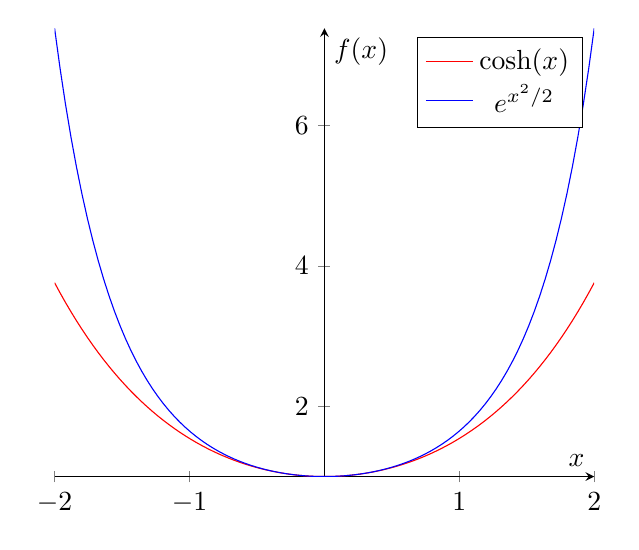
\begin{tikzpicture}
    \begin{axis}[
        axis lines = center,
        xlabel = $x$,
        ylabel = {$f(x)$},
    ]
    %Below the red parabola is defined
    \addplot [
        domain=-2:2, 
        samples=100, 
        color=red,
    ]
    {cosh(x)};
    \addlegendentry{$\cosh(x)$}
    %Here the blue parabloa is defined
    \addplot [
        domain=-2:2, 
        samples=100, 
        color=blue,
        ]
        {exp(x^2/2)};
    \addlegendentry{$e^{x^2/2}$}
    \end{axis}
    \end{tikzpicture}
\end{subfigure}
\end{figure}

% \begin{figure}[H]
%     \centering
%     \begin{tikzpicture}
%     \begin{axis}[
%         axis lines = center,
%         xlabel = $x$,
%         ylabel = {$f(x)$},
%     ]
%     %Below the red parabola is defined
%     \addplot [
%         domain=-2:2, 
%         samples=100, 
%         color=red,
%     ]
%     {x^x};
%     \addlegendentry{$x^x$}
%     %Here the blue parabloa is defined
%     \addplot [
%         domain=-2:2, 
%         samples=100, 
%         color=blue,
%         ]
%         {x};
%     \addlegendentry{$e^{x^2/2}$}
%     \end{axis}
%     \end{tikzpicture}
% \end{figure}





\newcommand{\erdosrenyi}{Erd\"{o}s-R\'{e}nyi }

\subsection{Applications: Random Graphs}

At the intersection of graph theory and probability lies the Erd\"{o}s-R\'{e}nyi model. It is one of the simplest random graphs. The model has $n$ vertices, and the vertices are connected with some probability $p$; we denote such a graph as $G(n, p).$ \\ 

As a brief analysis on the \erdosrenyi model, let us study the expected number of edges per vertex. For every vertex, there are $(n-1)$ possible edges. However, since there is a fixed probability, $p$, of having a connection between verticies, the number of edges per vertex may be modeled as a binomial random variable $D$. Therefore, using the expectation of a binomial random variable, the expected number of edges per vertex is $d = E[D] = (n-1)p$. \\ 

\begin{tcolorbox}
\begin{definition}[Dense Graph]
A random graph $G(n, p)$ is said to be relatively \textit{dense} if the expected degree of each vertex is $E[D]= d \gtrsim \log{n}. $
\end{definition}
\end{tcolorbox}


% =======================================
% Proposition: Regularity of Dense Graphs
% =======================================
\begin{tcolorbox}
\begin{proposition}[Regularity of Dense Graphs]
Consider a random graph $G\sim G(n, p)$ with the expected degree $E[D] = d: d\geq C\log{n}$, where $C$ is some fixed constant. It follows that there is a probability $1-\varepsilon$ that all vertices within $G$ have degrees between $(1-\varepsilon) d$ and $(1+\varepsilon) d$. 
\end{proposition}
\end{tcolorbox}

% =====
% PROOF
% =====
\begin{proof}
To begin, we will work with an individual vertex $i$ within the graph $G$. Recall that we have already noted that the number of edges per vertex $D_i \sim binomial(n-1, p)$. Equivalently, we may say that the number of edges per vertex is represented by $D_i \sim \sum_{i=1}^{n-1} X_i$ where $X_i \sim Bernoulli(p).$ Since we have shown that we are working with sums of Bernoulli random variables, we may use the Chernoff bound.  \\ 

Using the small-deviations representation of the Chernoff bound in Equation $\ref{eq:chernoff2}$, we obtain 
$$ P\left( |D_i - d| \geq \varepsilon d \right) \leq 2e^{-cd}. $$
Now, when we consider all vertices in the graph, we find that 
    \begin{align*}
    P\left( \exists i\leq n: |D_i - d| \geq \varepsilon d \right) &\leq \sum_{i=1}^{n}P\left( |D_i - d| \geq \varepsilon d\right) && \text{Union bound ???} \\ 
    &\leq n \cdot 2e^{-cd} && \text{Chernoff's inequality for each vertex} \\ 
    &= \frac{2n}{e^{cd}}  \\ 
    &\leq \varepsilon &&\text{for large enough $c$} 
    \end{align*}
With our goal now to take the complimentary event, we have 
    \begin{align*}
    P\left( \exists i\leq n: |D_i - d| \geq \varepsilon d \right) &\leq \varepsilon &&\text{from previous} \\ 
    -P\left( \exists i\leq n: |D_i - d| \geq \varepsilon d \right) &\geq -\varepsilon &&\text{multiply both sides by $-1$} \\ 
    1-P\left( \exists i\leq n: |D_i - d| \geq \varepsilon d \right) &\geq 1-\varepsilon &&\text{add $1$ to both sides} \\ 
    P\left( \forall i \leq n: |D_i - d| < \varepsilon d \right) &\geq 1-\varepsilon &&\text{definition of complement} 
    \end{align*}
    That is, for arbitrary probability, we can create bounds for the number of degrees per vertex in the random graph.  
\end{proof}


\begin{tcolorbox}
    \begin{definition}[Big O Notation]
    $f(x) = O(g(x)) \iff \lim_{x\to\infty} f(x)/g(x) = C$
    \end{definition}
%
    \begin{definition}[o Notation]
    $f(x) = o(g(x)) \iff \lim_{x\to\infty} f(x)/g(x) = 0$ 
    \end{definition}
\end{tcolorbox}


\begin{figure}[H]
        \centering
        \includegraphics[scale=0.6]{Chernoff_Vs_Hoeffding}
        \caption{Hoeffding's inequality is not as sensitive as Chernoff's bound for means. }
\end{figure}

\subsection{Sub-Gaussian Distributions}
The reader may notice that our discussions of concentration inequalities have been restricted to heavy assumptions -- assumptions that random variables are Bernoulli, Symmetric Bernoulli, or bounded. In this section, we will extend our results to a larger class of distributions called the sub-Gaussian distributions. We will then explore its properties.  

% ===============================
% Bounds on Gaussian Distribution
% ===============================
Before we continue further with discussion of Sub-Gaussian distributions, it is worthwhile to explore the bounds on the Gaussian distribution. \\

\begin{tcolorbox}
\begin{proposition}[Tails of the Normal Distribution]
Suppose $X \sim N(0,1)$. For $t > 0$, the tails of the normal distribution may be represented by 
$$ \left(\frac{1}{t} - \frac{1}{t^3} \right) \cdot \frac{1}{\sqrt{2\pi}} e^{-t^2/2} \leq P(X \geq t) \leq \frac{1}{t} \cdot \frac{1}{\sqrt{2\pi}} e^{-t^2/2}$$
\end{proposition}
\end{tcolorbox}

\begin{proof}
\noindent Upper Tail:  \\ 
Strategy: the objective of concentration inequalities is to get the inequalities to be functions of $t$. In other words, we want to get the concentration inequalities to illustrate probabilities as they deviate from the mean. In proofs, we will often simplify expressions using inequalities. However, we never want to simplify any term that includes $t$.    
    \begin{align*}
    P(X \geq t) &= \frac{1}{\sqrt{2\pi}} \int_{t}^{\infty} e^{-x^2/2}dx &&\text{} \\
    &= \frac{1}{\sqrt{2\pi}} \int_{t}^{\infty} e^{-(t+y)^2/2}dy &&\text{change of var: x = t+y} \\
    &= \frac{1}{\sqrt{2\pi}} \int_{t}^{\infty} e^{-t^2/2} e^{-ty} e^{-y^2/2}dy &&\text{} \\
    &= \frac{1}{\sqrt{2\pi}}e^{-t^2/2} \int_{t}^{\infty} e^{-ty} e^{-y^2/2}dy &&\text{since $e^{-t^2/2}$ is not a function of $y$} \\
    &\leq \frac{1}{\sqrt{2\pi}}e^{-t^2/2} \int_{t}^{\infty} e^{-ty}dy &&\text{since $e^{-y^2} < 1$ for $t \in (0, \infty)$ and $y \in [t,\infty)$} \\
    &= -\frac{1}{\sqrt{2\pi}}e^{-t^2/2} \frac{1}{t}e^{-ty}\Bigg|_{t}^{\infty} &&\text{take integral} \\
    &= 0 - \left( -\frac{1}{\sqrt{2\pi}}e^{-t^2/2} \frac{1}{t}e^{-ty} \right) &&\text{} \\
    &= \frac{1}{t} \cdot \frac{1}{\sqrt{2\pi}}e^{-t^2/2} e^{-t^2} &&\text{} \\
    &\leq \frac{1}{t} \cdot \frac{1}{\sqrt{2\pi}} e^{-t^2/2} &&\text{??? Why would we do this} \\
    \end{align*}
\end{proof}

\noindent 
Hoeffding's: $\displaystyle{P\left(\left|\sum_{i=1}^{N} a_i X_i\right| \geq t\right) \leq 2\exp\left( -\frac{t^2}{2 \|a\|_{2}^{2}}\right)}$ \\ 
Chernoff's: $\displaystyle{P\left(\left|\sum_{i=1}^{N}X_i - \mu\right| \geq \delta \mu\right) \leq 2 \exp{\{-c\mu \delta^2\}}}$ \\ 
Normal: $\displaystyle{ P\left(X \geq t \right) \leq \frac{1}{t}\cdot \frac{1}{\sqrt{2\pi}} \exp{\left(-\frac{t^2}{2}\right)} }$ \\ 

Taking a look at the bounds between Hoeffding's inequality and the bound on the normal distribution, there is clearly some similarities. This is a hint that there may be some underlying structure. The notion of sub-Gaussian distributions is a class of distributions where the probabilities in the tails converge at least as fast as the Gaussian distribution. 

To make this even clearer, we may observe that Hoeffding's inequality where $N=1$ results in 
$$ P\left( \left|X \right| \geq t\right) \leq 2\exp\left( -\frac{t^2}{2} \right). $$

\begin{tcolorbox}
\begin{proposition}[Sub-Gaussian Properties]
If $X$ is a random variable, such that $K_1, ..., K_5$ are all positive and are constants, then the following are equivalent 
    \begin{enumerate}
    \item $\displaystyle{ P\left( |X| \geq t \right) \leq 2 \exp\left( -t^2/K_1^2 \right) }$ for $t \geq 0$
    \item $\displaystyle{ \|X\|_{L^p} = \left( E\big[|X|^p\big] \right)^{1/p} \leq K_2\sqrt{p}}$ for $p \geq 1$
    \item The MGF of $X^2$ satisfies
    $$ \Expect{\exponential{\lambda^2 X^2}} \leq \exponential{K_3^2 \lambda^2} $$
    \item The MGF of $X^2$ is bounded at some point. In particular,
    $$ \Expect{\exponential{X^2/ K_4^2}} \leq 2. $$ 
    \item If $E[X] = 0$, then the MGF of $X$ satisfies
    $$ \Expect{\exponential{\lambda x}} \leq \exponential{K_5^2 \lambda^2} for \lambda \in \mathbb{R}$$
    \end{enumerate}
\textbf{Note:} Properties (1)-(5) are equivalent in the sense that there exists some absolute constant $C$, and property $i$ implies property $j$ such that $K_j \leq C K_i. $
\label{prop:subgaussian}
\end{proposition}
\end{tcolorbox}


% ===========
% Add Pictures
% ===========
\begin{figure}[H]
        \centering
        \includegraphics[scale=0.6]{Normal_vs_SubGaussian}
        \caption{Illustration that Sub-Gaussian distributions are \textit{below} the normal distribution -- hence the name. }
\end{figure}

% ============
% Proof 1 => 2
% ============
\begin{proof}
    %%%% 
    $(\text{Property }1 \implies \text{Property }2): $ \textcolor{orange}{Assume (1) is true.} 
    \begin{align*}
    %
    E\big[|X|^p\big] &= \int_{0}^{\infty} P\left(|X|^p \geq u\right)du && 
        \text{Integral Identity $\left(|X|^p \geq 0\right)$} \\ 
    &= \int_{0}^{\infty} \Prob{|X|^p \geq \textcolor{\darkgreen}{t^p} }du &&
        \text{Substitute: $u = t^p$} \\ 
    &= \int_{0}^{\infty} \Prob{ |X|^p \geq t^p }\textcolor{\darkgreen}{pt^{p-1}dt} && 
        \text{$du = pt^{p-1}dt$} \\ 
    &= \int_{0}^{\infty} \Prob{ \textcolor{\darkgreen}{|X| \geq t }}pt^{p-1}dt && 
        \text{$p$th root of both sides} \\ 
    &\leq \int_{0}^{\infty} \textcolor{\darkgreen}{2\exponential{-t^2}}pt^{p-1}dt &&
        \text{Property 1 \textcolor{orange}{assuming $K_1^2=1$}}  \\
    &= p \int_{0}^{\infty} 2t^{p-1} e^{-t^2} dt &&
        \text{Rearrange} \\ 
        %
    \end{align*}
    \textcolor{orange}{Recall} that the Gamma function is 
    \begin{align*}
        \Gamma(z) &= \int_{0}^{\infty} y^{z-1}e^{-y}dy 
            &&\text{defn. } \\ 
        &= \int_{0}^{\infty} \textcolor{\darkgreen}{t}^
            {\textcolor{\darkgreen}{2}(z-1)}e^{-t^2} dy
            &&\text{Substitute $y = t^2$} \\
        &= \int_{0}^{\infty} \textcolor{\darkgreen}{2t} t^{2(z-1)}e^{-t^2} \textcolor{\darkgreen}{dt}
            &&\text{$dy = 2tdt$} \\ 
        &= \int_{0}^{\infty} 2 t^{\textcolor{\darkgreen}{2z - 1}}e^{-t^2} dt
            &&\text{} \\ 
    \end{align*}
    \textcolor{orange}{Continuing on}, and using this representation, we find that 
    \begin{align*}
        \Expect{|X|^p} &\leq p \int_{0}^{\infty} 2t^{p-1} e^{-t^2} dt &&
            \text{From Above} \\ 
        &= p \int_{0}^{\infty} 2t^{\textcolor{\darkgreen}{2(p/2)}-1} e^{-t^2} dt &&
            \text{Rearrange} \\ 
        &= p \cdot \textcolor{\darkgreen}{\Gamma(p/2)} && 
            \text{Gamma Defn.} \\ 
        &\leq p \cdot \textcolor{\darkgreen}{(p/2)^{p/2}} &&
            \text{\textcolor{red}{$\Gamma(x) \leq x^x$ from Stirling Approx.}} \\ 
        \textcolor{\darkgreen}{\big(}\Expect{|X|^p}\textcolor{\darkgreen}{\big)^{1/p}} &\leq \textcolor{\darkgreen}{\big(}(p/2)^{p/2}\textcolor{\darkgreen}{\big)^{1/p}} &&
            \text{take $p$th root of both sides} \\ 
        &= (p/2)^{\textcolor{\darkgreen}{1/2}} &&
            \text{} \\ 
        &= \textcolor{\darkgreen}{K_2} \sqrt{p} && 
    \end{align*}
    %%%% 
\end{proof}

% ==============
% Proof Technique
% ==============
\begin{tcolorbox}[colback=white!90!gray, title=Proof Technique: Bounding $P$-Norm]
\begin{enumerate}
    \item Represent $\Expect{|X|^p}$ with integral identity
    \item Bind $\Expect{|X|^p}$ by sub-Gaussian tail from property 1
    \item Represent exponential tail as Gamma function
    \item Bind Gamma function with $\Gamma(x) \leq x^x$ to create bound dependent only on $p$ 
\end{enumerate}
\end{tcolorbox}


% ==============
% Proof: 2 => 3 
% ==============
\begin{proof}
(Property 2 $\implies$ Property 3): \textcolor{orange}{Assume (2) is true.}
\begin{align*}
M_{X^2}(\lambda^2) &= \Expect{e^{\lambda^2 X^2}} && 
    \text{\textcolor{red}{defn. of MGF of $X^2$} } \\ 
&= \Expect{\textcolor{\dgreen}{\sum_{p=0}^{\infty} \frac{(\lambda^2 X^2)^p}{p!}}} && 
    \text{summation notation of series expansion} \\ 
&= \sum_{p=0}^{\infty} \frac{\lambda^{2p} \textcolor{\dgreen}{\Expect{X^{2p}}}}{p!} &&
    \text{distribute expectation} \\ 
&\leq \sum_{p=0}^{\infty} \frac{ \lambda^{2p} \Expect{X^{2p} } }{\textcolor{\dgreen}{(p/e)^p}} &&
    \text{\textcolor{blue!50!white}{since $(p/e)^p \leq p!$}} 
\end{align*}
Notice that we have 
\begin{align*}
    \Expect{X^{2p}} &= \Expect{\textcolor{\dgreen}{|X|}^{2p}} && 
        \text{since $2p$ is always even} \\ 
    &\leq \left(K_2 \sqrt{2p} \right)^{2p} && 
        \text{$\Expect{|X|^q} \leq \left(K_2 \sqrt{q}\right)^q$ by prop. (2)} \\ 
    &= K_2^{2p} \left(2p \right)^p && 
        \text{} \\ 
    &= (2p)^p && \text{\textcolor{orange}{let $K_2 = 1$}}. 
\end{align*}
Substituting this inequality back into the bound on the MGF, we obtain 
\begin{align*}
    M_{X^2}(\lambda^2) &\leq \sum_{p=0}^{\infty} \frac{ \lambda^{2p} \textcolor{\dgreen}{(2p)^p} }{ (p/e)^p } && 
        \text{substitute $\Expect{X^{2p}} \leq (2p)^p$} \\ 
    &= \sum_{p=0}^{\infty} \textcolor{\dgreen}{(2\lambda^2 e)^p} && 
        \text{} 
\end{align*}
\textcolor{orange}{Recall} that the geometric series states that for $-1 < r < 1$, $\sum_{k=0}^{\infty} r^k = \frac{1}{1-r}.$ It follows now that 
\begin{align*}
    M_{X^2}(\lambda^2) &\leq \textcolor{\dgreen}{\frac{1}{1 - 2\lambda^2 e}} &&\text{ for $-1 < 2\lambda^2 e < 1$} &&& \text{geometric series} \\ 
    & &&\text{ for } \textcolor{\dgreen}{|\lambda| \leq \sqrt{\frac{1}{2e}}} &&&  \\
    &\leq \textcolor{\dgreen}{e^{4 \lambda^2 e}} &&\text{ for $0 \leq 2\lambda^2 e \leq 1/2$} &&& 
        \text{since \textcolor{blue!50!white}{$\frac{1}{1-x} \leq e^{2x}$ for $0 \leq x \leq 1/2$}} \\ 
    & && \text{ for } \textcolor{\dgreen}{|\lambda| \leq \frac{1}{2 \sqrt{e}}}
\end{align*}
\end{proof}

% ==============
% Proof Technique
% ==============
\begin{tcolorbox}[colback=white!90!gray, title=Proof Technique: Bounding MGF of $X^2$]
\begin{enumerate}
    \item represent series expansion of $X^2$ MGF with summation notation 
    \item apply inequalities to bind series expansion of $X^2$ MGF with geometric series
    \item bind geometric series by exponential tail 
\end{enumerate}
\end{tcolorbox}

% =============
% Proof: 3 => 4
% =============
\begin{proof}
(Property 3 $\implies$ Property 4): \textcolor{orange}{Assume (3) is true}.
We know that 
\begin{align*}
    \Expect{\lambda^2 \exponential{X^2}} &\leq \exponential{K_3^2 \lambda^2} && |\lambda| \leq \frac{1}{K_3} &&& \text{Prop. 3} \\
    & && \lambda^2 \leq \frac{1}{K_3^2} &&&  \\
    \implies \Expect{\exponential{X^2/\textcolor{\dgreen}{K_3^2}}} &\leq \exponential{K_3^2 / \textcolor{\dgreen}{K_3^2}} = e && &&& \text{for $\lambda^2 = 1/K_3^2$} 
\end{align*}
If we choose a $K_4 > K_3$, then the tail is bounded even further.  \\ 
\end{proof}

% ============
% Proof 4 => 1
% ============
\begin{proof}
(Property 4 $\implies$ Property 1): \textcolor{orange}{Assume (4) is true and $K = 1$}. It follows that 
\begin{align*}
    \Prob{|X| \geq t} &= \Prob{|X^{\textcolor{\dgreen}{2}}| \geq t^{\textcolor{\dgreen}{2}}} && 
        \text{square both sides} \\ 
    &= \Prob{\textcolor{\dgreen}{e}^{x^2} \geq \textcolor{\dgreen}{e}^{t^2}} &&
        \text{exponentiate both sides} \\ 
    &\leq \frac{E[\textcolor{\dgreen}{e}^{x^2}]}{\textcolor{\dgreen}{e}^{t^2}} &&
        \text{Markov's Inequality} \\ 
    &\leq 2e^{-t^2} &&
        \text{Property 4: $E[e^{x^2/k^2}] \leq 2$}
\end{align*}
\end{proof}

% ==============
% Proof Technique
% ==============
\begin{tcolorbox}[colback=white!90!gray, title=Proof Technique: Bounding Tail Decay]
\begin{enumerate}
    \item bound MGF with Markov's Inequality
    \item Apply MGF boundedness property to bound tail decay
\end{enumerate}
\end{tcolorbox}


% =============
% Proof 3 => 5 
% =============
\begin{proof}
(Property 3 $\implies$ Property 5): \textcolor{orange}{Assume (3) is true.}  \\ 


\noindent Case 1:$|\lambda| \leq 1$. \\
\noindent Notice that \textcolor{\lblue}{$e^x \leq x + e^{x^2/2}$ for all $x \in \mathbb{R}$}. It follows that 
\begin{align*}
    \Expect{e^{\lambda X}} &\leq \Expect{\lambda X + \exponential{\lambda^2 X^2 / 2}} &&
        \text{$e^x \leq x + e^{x^2/2}$} \\ 
    &= \lambda \Expect{X} + \Expect{\exponential{\lambda^2 X^2 /2 }} && 
        \text{distribute expectation} \\ 
    &= 0 + \Expect{\exponential{\lambda^2 X^2 /2 }} && 
        \text{since $E[X] = 0$ by hypothesis} \\ 
    &\leq \exponential{K^2 \lambda^2} && 
        \text{Property 3}
\end{align*}

\noindent Case 2: $|\lambda| \geq 1$.  \\
\noindent Notice that \textcolor{\lblue}{$2\lambda x \leq \lambda^2 + x^2$ for all $x \in \mathbb{R}$}. Under further analysis, we have 
\begin{align*}
2\lambda x &\leq \lambda^2 + x^2  \\
\implies e^{\lambda x} &\leq e^{\frac{\lambda^2 + x^2}{2}}. 
\end{align*}
It follows that 
\begin{align*}
    \Expect{e^{\lambda X}} &\leq \Expect{e^{\frac{\lambda^2+X^2}{2}}} && 
        \text{$2\lambda x \leq \lambda^2 + x^2$} \\ 
    &= e^{\lambda^2/2} \Expect{e^{X^2/2}} \\ 
    &\leq e^{\lambda^2/2} \textcolor{\dgreen}{e^{1/2}} &&\text{Prop. 3: $\Expect{e^{\lambda x}} \leq e^{1/2}$ for $K=1$} \\ 
    &= e^{\frac{\lambda^2+1}{2}} && \text{} \\ 
    &\leq e^{\lambda^2} && \text{$\lambda \geq 1 \implies \lambda^2 \geq 1 \implies$} \\ 
    & && \text{$\lambda^2+1 \geq 2 \implies  \frac{\lambda^2+1}{2} \geq 1$}
\end{align*}
\end{proof}

\begin{figure}[H]
\begin{subfigure}{0.5\textwidth}
    \centering
    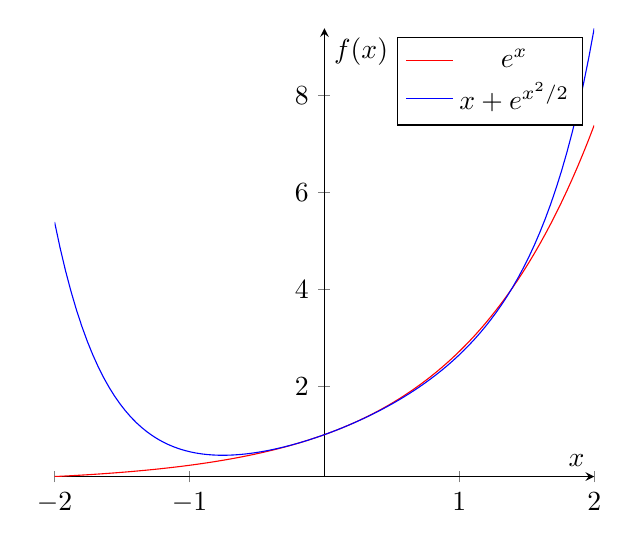
\begin{tikzpicture}
    \begin{axis}[
        axis lines = center,
        xlabel = $x$,
        ylabel = {$f(x)$},
    ]
    %Below the red parabola is defined
    \addplot [
        domain=-2:2, 
        samples=100, 
        color=red,
    ]
    {e^x};
    \addlegendentry{$e^x$}
    %Here the blue parabloa is defined
    \addplot [
        domain=-2:2, 
        samples=100, 
        color=blue,
        ]
    {x + exp(x^2/2)};
    \addlegendentry{$x + e^{x^2/2}$}
    \end{axis}
    \end{tikzpicture}
\end{subfigure}
\begin{subfigure}{0.5\textwidth}
    \centering
    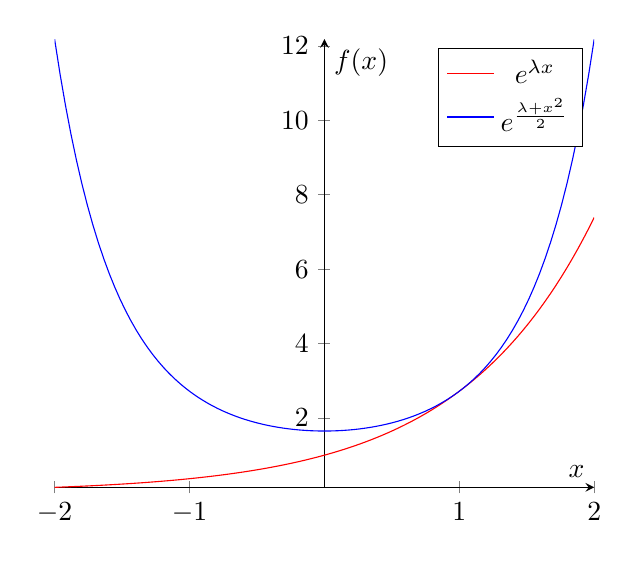
\begin{tikzpicture}
    \begin{axis}[
        axis lines = center,
        xlabel = $x$,
        ylabel = {$f(x)$},
    ]
    %Below the red parabola is defined
    \addplot [
        domain=-2:2, 
        samples=100, 
        color=red,
    ]
    {exp(x)};
    \addlegendentry{$e^{\lambda x}$}
    %Here the blue parabloa is defined
    \addplot [
        domain=-2:2, 
        samples=100, 
        color=blue,
        ]
    {exp(1/2+x^2/2)};
    \addlegendentry{$e^{\frac{\lambda + x^2}{2}}$}
    \end{axis}
    \end{tikzpicture}
\end{subfigure}
\end{figure}




% ==============
% Proof: 5 => 1 
% ==============
\begin{proof}
(Property 5 $\implies$ Property 1): \textcolor{orange}{Assume (5) is true and $E[X]=0.$}
\begin{align*}
    \Prob{X \geq t} &= \Prob{e^{\lambda x} \geq e^{\lambda t}} && \text{} \\
    &\leq \textcolor{\dgreen}{e^{-\lambda t} \Expect{e^{\lambda x}}} &&
        \text{Markov's Inequality} \\ 
    &\leq e^{-\lambda t} \textcolor{\dgreen}{\exponential{K^2 \lambda^2}} &&
        \text{Prop. 5: $\Expect{e^{\lambda x}} \leq \exponential{K^2 \lambda^2}$} \\ 
    &= \exponential{K^2 \lambda^2 - \lambda t} 
\end{align*}
Now, optimizing the bound to obtain the smallest upper bound, we have 
\begin{align*}
    \frac{d}{d \lambda} \left(\exponential{-\lambda t + K^2 \lambda^2 }\right) &= \exponential{-\lambda t + K^2\lambda^2} \left( -t + 2K^2 \lambda \right) && \text{product rule} \\  
    \implies 2 \lambda K^2 \exponential{-\lambda t + K^2 \lambda} &= t \exponential{-\lambda t + K^2 \lambda} \\ 
    \implies 2 \lambda K^2 &= t   \\
    \implies \lambda &= t/2K^2 \\ 
    \implies \lambda &= t/2 && \text{\textcolor{orange}{Let K =1}}
\end{align*}
Plugging $\lambda$ back into the bound, we obtain
\begin{align*}
    \Prob{X \geq t} &\leq \exponential{\textcolor{\dgreen}{t^2/4 - t^2/2}} && \text{$\lambda = t/2$} \\ 
    &= \exponential{-t^2/4} \\
    &= \exponential{-t^2/K^2} && \text{for $K = 2$} 
\end{align*}
\end{proof}

\begin{tcolorbox}
\begin{example}[Property 5 without 0 Mean]
Show that Property 5 does not hold if $E[X] \neq 0.$ \\ 
\end{example}
\end{tcolorbox}
\begin{proof}
\textcolor{orange}{Assume that Property 3 holds. } 
\begin{align*}
    \Expect{e^{\lambda X}} &\leq \Expect{\lambda X + e^{\lambda^2 X^2}} && 
        \text{$e^x \leq x + e^{x^2}$} \\ 
    &= \lambda \Expect{X} + \Expect{e^{\lambda^2 X^2}} && \text{} \\
    &\leq \lambda \Expect{X} + \exponential{\lambda^2 K^2}
\end{align*}
Since $\lambda \geq 0$, and $E[X] \neq 0$, for the case that $E[X] < 0$, the bound will be tighter than it should be. Also notice, that we cannot change the value of $K$ because $K$ is related to the absolute constant $C$, which is unchanging. 
\end{proof}



% Definition: Sub-Gaussian Random Variables
\begin{tcolorbox}
\begin{definition}[Sub-Gaussian Random Variable]
A random variable is said to be \textit{sub-gaussian} if it satisfies one of the four properties in Proposition \ref{prop:subgaussian}. Furthermore, we define the sub-gaussian norm as 
    \begin{equation}
    \|X\|_{\psi_2} = \inf\left\{ t>0: \Expect{\exponential{X^2/t^2}} \leq 2 \right\} \\
    \end{equation}
\end{definition}
\end{tcolorbox}

The properties in Proposition \ref{prop:subgaussian} \textit{feel} arbitrary because of the $K$ constants. There exists some absolute constant $C$ that relates all of the $K$ constants together, but the inequalities posed in Proposition \ref{prop:subgaussian} do not illustrate this connection. However, it turns out that we can rewrite the properties in terms of the sub-gaussian norm, resulting in more expressive forms -- illustrating the underlying relationship with $C$: \\ 

\begin{tcolorbox}[colback=white!90!gray, title=Proposition \ref{prop:subgaussian} With Sub-Gaussian Norm]
For $c>0$, and $C$ an absolute constant, 
    \begin{align}
    \Prob{|X| \geq t} &\leq 2 \exponential{-ct^2 / \|X\|^2_{\psi_2}} &&\text{ for $t\geq 0$} \\ 
    \|X\|_{L_p} &\leq C \|X\|_{\psi_2} \sqrt{p} &&\text{ for $p \geq 1$} \\ 
    \Expect{\exponential{X^2 / \|X\|^2_{\psi_2}}} &\leq 2  \\ 
    \text{if $E[X]=0$, } \Expect{\exponential{\lambda X}} &\leq \exponential{\left(C \lambda^2 \|X\|_{\psi^2}^{2} \right)} && \text{ for $\lambda \in \mathbb{R}$}
    \end{align}
\end{tcolorbox}




\subsection{General Hoeffding's and Khintchine's Inequalities}
In this section, we will generalize Hoeffding's inequality. So far, we have only been able to apply Hoeffding's inequality on bounded random variables. We will extend Hoeffding's inequality to sub-gaussian random variables with 0 mean in this section. Since we have now developed the theory for sub-gaussian random variables, we will utilize the theoretical developments of sub-gaussian random variables to avoid the usage of esoteric inequalities in the generalization of Hoeffding's inequality. \\

\begin{tcolorbox}
\begin{proposition}[Sums of Independent Sub-Gaussians]
Let $X_1, ..., X_N$ be independent sub-gaussian random variables. It follows that 
\begin{enumerate}
    \item $\displaystyle{S_n = \sum_{i=1}^{N} X_i \sim subgaussian}$
    \item $\displaystyle{\left\|\sum_{i=1}^{N}X_i \right\|_{\psi_2}^2 \leq C \sum_{i=1}^{N}\|X_i\|^2_{\psi_2} }$
\end{enumerate}
\label{prop:subg_sum}
\end{proposition}
\end{tcolorbox}

% ======
% Proof 
% ======
\begin{proof}
To begin, we will study the MGF of the sum. 
\begin{align*}
    M_{S_n}\lambda &= \Expect{\exponential{\lambda S_n}} && 
        \text{MGF defn.}  \\ 
    &= \Expect{\exponential{\lambda \sum_{i=1}^{N} X_i}} && 
        \text{$S_n = \sum_{i=1}^{N}X_i$} \\ 
    &= \prod_{i=1}^{N} \Expect{\exponential{\lambda X_i}} &&
        \text{$X_i$ independent}  
\end{align*}
Notice that for an individual $X_i$, it is sub-gaussian. That is 
\begin{align*}
    M_{X_i}(\lambda) &= \Expect{\exponential{\lambda X_i}} &&
        \text{MGF defn.} \\ 
    &\leq \exponential{C \lambda^2 \|X_i\|_{\psi_2}^2} &&
        \text{normed sub-gaussian property 5} \\ 
\end{align*}
Plugging this inequality back into the MGF of $S_n$ we obtain
\begin{align*}
    M_{S_n}(\lambda) &\leq \prod_{i=1}^{N} \exponential{C \lambda^2 \|X_i\|_{\psi_2}^{2}} && \\ 
    &= \exponential{C \lambda^2 \sum_{i=1}^{N}\|X_i\|_{\psi_2}^2} && \text{exponential property} \\ 
    &= \exponential{\lambda^2 K^2} && \text{Let $K^2 = C \sum_{i=1}^{N} \|X_i\|_{\psi_2}^{2}$}  
\end{align*}
It is clear that $S_n$ follows sub-gaussian property 5. Therefore, it follows that $S_n$ is also sub-gaussian. \\
%
\textcolor{red}{Now, we also see that}
\begin{align*}
    \left\|\sum_{i=1}^{N}X_i\right\|_{\psi_2} &\leq C_1 K \\ 
    &= C_1 \sqrt{\sum_{i=1}^{N} \|X_i\|_{\psi_2}^2} \\ 
    \implies \left\|\sum_{i=1}^{N}X_i\right\|_{\psi_2}^2 &\leq C_1^2 \sum_{i=1}^{N} \|X_i\|_{\psi_2}^2 \\ 
\end{align*}
\end{proof}

% ============================
% Theorem: General Hoeffding's
% ============================
\begin{tcolorbox}
\begin{theorem}[General Hoeffding's Inequaliity for Subgaussian Random Variables]
Suppose $X_1, ..., X_n$ are independent sub-gaussian random variables with mean 0. 
\end{theorem}
\end{tcolorbox}

\begin{align*}
    S_n \text{ is sub-gaussian }& && \text{Proposition \ref{prop:subg_sum}} \\ 
    \implies P\left(\left| \sum_{i=1}^{N} X_i \right| \geq t \right) &\leq 2 \exponential{\frac{-Ct^2}{\left\|\sum_{i=1}^{N} X_i\right\|_{\psi_2}^2}} && 
        \text{normed sub-gaussian prop. 1} \\ 
    P\left(\left| \sum_{i=1}^{N} X_i \right| \geq t \right) &\leq 2 \exponential{\frac{-Ct^2}{\textcolor{\dgreen}{\sum_{i=1}^{N}\left\| X_i\right\|_{\psi_2}^2}}} && \text{since $\left\| \sum_{i=1}^{N} X_i \right\| \leq C\sum_{i=1}^{N} \|X_i\|_{\psi_2}^{2}$}
\end{align*}


\begin{tcolorbox}
\begin{theorem}[Khintchine's Inequality]
Let $X_1, ..., X_n$ be sub-gaussian random variables with 0 mean, and unit variance. For $(a_1, ..., a_n) \in \mathbb{R}^n$ and $p \in [2, \infty]$, it follows that 
$$ \left(\sum_{i=1}^{N}a_i^2 \right)^{1/2} \leq \left\| \sum_{i=1}^{N}a_i X_i \right\|_{L_p} \leq C K \sqrt{p} \left(\sum_{i=1}^{N} a_i^2 \right)^{1/2} $$
\end{theorem}
\end{tcolorbox}


\subsection{Centering}
Concentration inequalities are fundamentally  about how far a random variable may differ from the mean. For convenience, we often assume that random variables have mean 0. Fortunately, if a random variable does not have mean 0, the concentration inequalities that we have developed are unaffected once we center them. 

\begin{tcolorbox}
\begin{example}
    Show that the following centering inequality for the $L^2$ norm holds. 
    $$\|X - \Expect{X} \|_{L^2} \leq \|X\|_{L^2}$$
\end{example}
\end{tcolorbox}

\begin{tcolorbox}
\begin{lemma}[Centered Sub-Gaussian RVs are Sub-Gaussian]
Suppose $X$ is a sub-gaussian random variable. It follows that $X - \Expect{X}$ is also sub-gaussian. That is, 
$$\|X - \Expect{X} \|_{\psi_2} \leq C \|X\|_{\psi_2}$$
\end{lemma}
\end{tcolorbox}

\begin{proof}
\begin{align*}
    \|X - \Expect{X}\|_{\psi_2} &\leq \|X\|_{\psi_2} + \|\Expect{X}\|_{\psi_2} && \text{Triangle Inequality for Norms}\\ 
    &\leq \|X\|_{\psi_2} + \textcolor{\dgreen}{C|\Expect{X}|} && \text{$\|\Expect{X}\|_{\psi_2} \leq C|X|$ for large $C$} \\
    &\leq \|X\|_{\psi_2} + C \textcolor{\dgreen}{\Expect{|X|}} && \text{Jensen's Inequality: $f(\Expect{X}) \leq \Expect{f(X)}$} \\ 
    &= \|X\|_{\psi_2} + C \textcolor{red}{\|X\|_1} && \\
    &= \|X\|_{\psi_2} + C' \|X\|_{\psi_2} && \text{Property 2: $\|X\|_{L^p} \leq C \|X\|_{\psi_2}\sqrt{p}$ for $p=1$}\\ 
    &= C''\|X\|_{\psi_2} 
\end{align*}
\end{proof}







\subsection{Sub-Exponential Distributions}
We have considered a large class of distributions that contains useful inequalities -- the sub-gaussian distributions. Now, we turn our attention to a secondary class of distributions -- the sub-exponential distributions. Although the sub-gaussian class contains the most important distributions, the sub-exponential class also contains many useful distributions as well. To illustrate, suppose $g_i \sim N(0, 1),$ and therefore, sub-gaussian. As it turns out though, $g_i^2$ is not sub-gaussian. 

\begin{align*}
    \Prob{g_i^2 > t} &= \Prob{\textcolor{\dgreen}{|g_i|} > \textcolor{\dgreen}{\sqrt{t}}} && \text{take square root} \\
    &\leq \textcolor{\dgreen}{2\exponential{-(\sqrt{t})^2/2}} && 
        \text{by exponential tail} \\ 
    &= 2\exponential{-\textcolor{\dgreen}{t}/2}
\end{align*}
Therefore, the sum of squared normal random variables is not sub-gaussian, but sub-exponential.  \\

\begin{tcolorbox}
\begin{proposition}[Sub-Exponential Properties]
If $X$ is a random variable, then the following are equivalent, differing by at most, some constant factor. 
\begin{enumerate}
    \item The tails of $X$ satisfy
        $$ \Prob{|X| \geq t} \leq 2 \exponential{-t/K_1} \text{ for $t \geq 0$.} $$
    \item The moments of $X$ satisfy
        $$ \|X\|_{L^p} = \left(E[|X|]^p \right)^{1/p} \leq K_2 p \text{ for $p \geq 1$.} $$
    \item The MGF of $|X|$ satisfies
        $$\Expect{\exponential{\lambda |X|}} \leq \exponential{K_3 \lambda} \text{ for all $0 \leq \lambda \leq 1/K_3$}$$
    \item The MGF of $|X|$ is bounded at some point
        $$ \Expect{\exponential{|X|/K_4}} \leq 2.$$
\end{enumerate}
\label{prop:subexp}
\end{proposition}
\end{tcolorbox}

% PROOF: Property 2 => 5
\begin{proof}
Property $(2 \implies 5):$
\begin{align*}
    \Expect{\exponential{\lambda X}} &= \Expect{1 + \lambda x + \frac{\lambda^2 x^2}{2!} + ...} && \text{series expansion} \\ 
    &= 1 + \lambda \Expect{X} + \sum_{p=2}^{\infty} \frac{\lambda^p \Expect{X}^p}{p!} \\
    &= 1 + \sum_{p=2}^{\infty} \frac{\lambda^p \Expect{X}^p}{p!} && \text{$\Expect{X} = 0$} \\ 
    &\leq 1 + \sum_{p=2}^{\infty} \frac{\lambda^p p^p}{p!} && \text{Prop. 2: } \Expect{|X|}^p \leq p^p \\
    &\leq 1 + \sum_{p=2}^{\infty} \frac{\lambda^p p^p}{(p/e)^p} && \text{Stirling: } p! \geq (p/e)^p \\ 
    &= 1 + \sum_{p=2}^{\infty} \left(\frac{\lambda p}{(p/e)}\right)^p \\
    &= 1 + \sum_{p=2}^{\infty} \left(\lambda e\right)^p \\
    &= 1 + \frac{(\lambda e)^2}{1 - \lambda e} \text{ for $|\lambda e|<1$} && \text{Geometric Series}
\end{align*}
The result becomes more beautiful if we tighten the geometric series a little further. That is, for $|\lambda e| < 1/2$, or equivalently for $2|\lambda e| < 1$, we have
\begin{align*}
    \Expect{\exponential{\lambda X}} &\leq 1 + \frac{(2\lambda e)^2}{1-2\lambda e} && \text{} \\ 
    &= \frac{1 - 2\lambda e +  (2\lambda e)^2}{1-2\lambda e} \\ 
    &= 1 - 2\lambda e
\end{align*}
\end{proof}

% =================
% Property (5 => 2)
% =================
\begin{proof}
Assume property 5 is true. It follows that  
\begin{align*}
\textcolor{purple}{|x|^p} &\textcolor{purple}{\leq p^p (e^x + e^{-x})} && \text{given inequality} \\ 
\Expect{|X|^p} & \leq \Expect{p^p(e^X + e^{-X})} && \text{let $X = x$ and take expectation} \\ 
&= p^p (\Expect{e^X} + \Expect{e^{-X}}) \\
\end{align*}
Notice that from property 5, and with a small enough $K_1$, $\Expect{e^{K_1 X}} \leq 1$ and for big enough $K_2$ $\Expect{e^{-K_2 X}} \leq 1$. Therefore, we have 
\begin{align*}
\Expect{|X|^p} &\leq 2p^p \\ 
\implies (\Expect{|X|^p})^{1/p} &\leq K p. \\ 
\end{align*}
\end{proof}






\begin{tcolorbox}
\begin{definition}[Sub-Exponential Random Variable]
A random variable is said to be sub-exponential if it satisfies one of the four properties in Proposition \ref{prop:subexp}. Furthermore, we define the sub-gaussian norm as 
\begin{equation}
    \|X\|_{\psi_1} = \inf\{t > 0: \Expect{|X|/t \leq 2}\}
\end{equation}
\end{definition}
\end{tcolorbox}


\begin{tcolorbox}
\begin{lemma}[Sub-Exponential RV is Sub-Gaussian RV Squared]
If $X$ is a sub-gaussian random variable if and only if $X^2$ is sub-exponential. More precisely,
$$\|X^2\|_{\psi_1} = \|X\|_{\psi_2}^2$$
\end{lemma}
\end{tcolorbox}

\begin{proof}
Notice the following definitions:
\begin{align*}
    \|X\|_{\psi_2} &= \inf\left\{ t > 0: \Expect{\exponential{X^2/t^2}}\leq 2 \right\}  && \text{sub-gaussian defn. of $X^2$} \\
    \|X^2\|_{\psi_1} &= \inf\left\{ s > 0: \Expect{\exponential{X^2/s}}\leq 2 \right\}  && \text{sub-exponential defn. of $X$} 
\end{align*}
Notice, that if $s = t^2$, then the definitions become equivalent, and thus $\|X^2\|_{\psi_1} = \|X\|_{\psi_2}^2.$
\end{proof}


\begin{tcolorbox}
\begin{lemma}[Product of Sub-Gaussians Is Sub-Exponential]
If $X$ and $Y$ are sub-gaussian random variables, then $XY$ is a sub-exponential random variable. In particular, we obtain the following relationship:
\begin{align*}
    \|XY\|_{\psi_1} &\leq \|X\|_{\psi_2} \|Y\|_{\psi_2} \\ 
\end{align*}
\end{lemma}
\end{tcolorbox}

\begin{proof}
\begin{align*}
XY &\leq X^2/2 + Y^2/2 && \text{Young's Inequality} \\ 
\Expect{XY} &\leq \Expect{\exponential{X^2/2 + Y^2/2}} && \text{} \\ 
&= \Expect{\exponential{X^2/2} \exponential{Y^2/2}} && \text{} \\ 
&\leq \Expect{\frac{\exponential{(X^2/2)}^2}{2} + \frac{\exponential{(Y^2/2)}^2}{2}} && \text{Young's Inequality} \\
&= \frac{1}{2} \Expect{\exponential{X^2} + \exponential{Y^2}} \\ 
&= \frac{1}{2} \left(\Expect{\exponential{X^2}} + \Expect{\exponential{Y^2}}\right) \\ 
&\leq \frac{1}{2} \left(2 + 2\right) = 2 && \text{SubGauss. Prop. 4}
\end{align*}
\end{proof}


\begin{tcolorbox}
\begin{theorem}[Bernstein's Inequality]
Let $X_1, ..., X_N$ be independent sub-exponential random variables with mean 0. For $a = (a_1, .., a_N) \in \mathbb{R}^N$, $K = \max_i \|X_i\|_{\psi_1}$, and $t \geq 0, $
\begin{equation}
    \Prob{\left|\sum_{i=1}^{N}a_i X_i\right| \geq t} \leq 2\exponential{-c \min\left(\frac{t^2}{K^2\|a\|_{2}^{2}}, \frac{t}{K \|a\|_{\infty}}\right)}
\end{equation}
In particular, for $a_i = 1/N, $ we have
\begin{equation}
    \Prob{\left|\frac{1}{N} \sum_{i=1}^{N} X_i\right| \geq t} \leq 2\exponential{-c\cdot N \min\left(\frac{t^2}{K^2}, \frac{t}{K}\right)}
\end{equation}
\end{theorem}
\end{tcolorbox}


% \begin{tcolorbox}
% \begin{theorem}[Bennett's Inequality]
% Let $X_1, ...,, X_N$ be independent random variables. Let $\sigma^2 = \sum_{i=1}^{N}Var(X_i)$ and $h(u) = (1+u)\log(1 + u) - u$. Further, assume $|X_i - \Expect{X_i}| \leq K$ almost surely. It follows that for $t > 0$
%     \begin{equation}
%     \Prob{\sum_{i=1}^{N} (X_i - \Expect{X_i}) \geq t} \leq \exponential{-\frac{\sigma^2}{K^2} h\left(\frac{Kt}{\sigma^2}\right)}
%     \end{equation}
% \end{theorem}
% \end{tcolorbox}



% ============================================
% Chapter 3: Random Vectors in High Dimensions
% ============================================
\pagebreak


% ================================
% Random Vectors in High Dimension
% ================================
\begin{figure}[H]
\centering
\begin{tikzpicture}[scale=2.0]

% Draw Square 
\draw[] (0, 0) -- (0, 2) -- (2, 2) -- (2, 0) -- (0, 0);
\draw[dashed] (0.5, 0.5) -- (0.5, 2.5) -- (2.5, 2.5) -- (2.5, 0.5) -- (0.5, 0.5);
\draw[] (2, 2) -- (2.5, 2.5);
\draw[dashed] (0, 0) -- (0.5, 0.5);
\draw[] (2, 0) -- (2.5, 0.5);
\draw[] (0, 2) -- (0.5, 2.5);

\draw[] (0, 0) -- (0, 1) -- (1, 1) -- (1, 0) -- (0, 0);
\draw[dashed] (0.25, 0.25) -- (0.25, 1.25) -- (1.25, 1.25) -- (1.25, 0.25) -- (0.25, 0.25);
\draw[dashed] (1, 1) -- (1.25, 1.25);
\draw[dashed] (0, 0) -- (0.25, 0.25);
\draw[dashed] (1, 0) -- (1.25, 0.25);
\draw[dashed] (0, 1) -- (0.25, 1.25);

\draw[] (0.9, -0.1) -- (1.1, 0.1) node[at start, below] {1};
\draw[] (1.9, -0.1) -- (2.1, 0.1) node[at start, below] {2};
\end{tikzpicture}
\end{figure}


\section{Random Vectors in High Dimensions}
So far, we have covered numerous probability bounds on individual random variables, as well as sums of random variables. Now, we will turn our attention towards random vectors. The driving motivation of extending our theory to random vectors in high dimension is evident based on the typical problems faced in data science. Unlike problems in the past where an outcome could be well estimated with a few covariates, problems in the 21st century must be estimated with thousands of covariates. 

Unfortunately, due to the high dimensionality of today's problems, classical tools in statistics become infeasible to use -- this is dubbed the \textit{curse of dimensionality}. To illustrate why classical tools become infeasible is 



\subsection{Concentration of the Norm}

% =======================================
% Illustration: Concentration of the Norm
% =======================================
\begin{figure}[H]
\centering
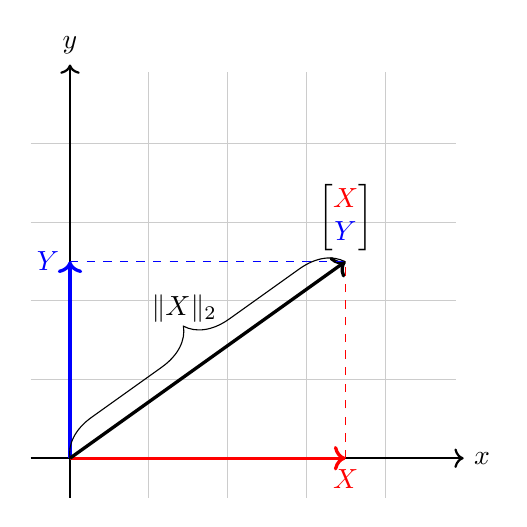
\begin{tikzpicture}

    % Draw Grid
    \draw[very thin, gray!40!white] (-0.5, -0.5) grid (4.9, 4.9); % Grid 
    \draw[thick, ->] (-0.5, 0) -- (5, 0) node[anchor=west] {$x$};
    \draw[thick, ->] (0, -0.5) -- (0, 5) node[anchor=south] {$y$};
    
    \draw[very thick, ->, red] (0, 0) -- (3.5, 0) node[anchor=north] {$X$};
    \draw[very thick, ->, blue] (0, 0) -- (0, 2.5) node[anchor=east] {$Y$};
    \draw[very thick, ->] (0, 0) -- (3.5, 2.5) node[anchor=south] {$\left[ \begin{matrix} \textcolor{red}{X} \\ \textcolor{blue}{Y} \end{matrix} \right]$};
    
    \draw[thin, dashed, red] (3.5, 0) -- (3.5, 2.5); 
    \draw[thin, dashed, blue] (0, 2.5) -- (3.5, 2.5); 
    
    % Label Norm
    \draw[decorate, decoration={brace, amplitude=15pt}] (0, 0) -- (3.5, 2.5) node[anchor=south, midway, xshift=-0.3cm, yshift=0.35cm] {$\|X\|_2$};
\end{tikzpicture}
\caption{Curse of Dimensionality}
\end{figure}


% =======
% Theorem: Concentration of Norm
% =======
\begin{remark}[Expected Length of $n$-Dimensional Vector]
Suppose we have an $n$-dimensional vector $X = (X_1, ..., X_n). $ Suppose further that each $X_i$ has mean 0, and variance 1. In order to find the squared norm of $X$, we have
\begin{align*}
    \Expect{\|X\|^2_2} &= \Expect{\sum_{i=1}^{n} X_i^2} && \text{defn. norm} \\ 
    &= \sum_{i=1}^{n} \Expect{X_i^2} && \text{since $X_i$ independent.} \\ 
    &= \sum_{i=1}^{n} 1 && \text{$\Expect{X_i} = 0 \implies Var(X_i) = \Expect{X_i^2} = 1$} \\ 
    &= n
\end{align*}
Therefore, the expected squared euclidean norm of $X$ is $n$, or in other words, the norm of $X$ should be around $\sqrt{n}.$ Although the expected norm is $\sqrt{n}$, we will now turn our attention towards the question of how close the vector will be to its norm. 
\end{remark}

% Drawing Sphere
\begin{figure}[H]
\centering
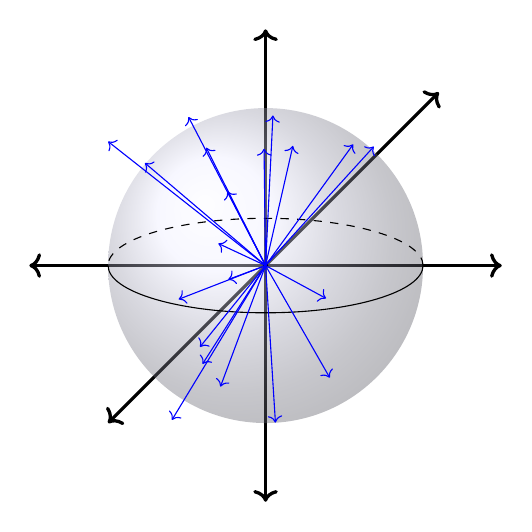
\begin{tikzpicture}

    % Draw Grid
    \draw[very thick, <->] (0,-3) -- (0, 3);
    \draw[very thick, <->] (-3,0) -- (3, 0);
    \draw[very thick, <->] (-2, -2) -- (2.2, 2.2);

    % Draw Sphere
    \shade[ball color = blue!10, opacity = 0.4] (0,0) circle (2cm); % Shade Sphere
    \draw (-2,0) arc (180:360:2 and 0.6);                           % Draw Front Circumference
    \draw[dashed] (2,0) arc (0:180:2 and 0.6);                      % Draw Back Circumference
    \fill[fill=black] (0,0) circle (1pt);                           % Draw Center
%  \draw[dashed] (0,0 ) -- node[above]{$r$} (2,0);                 % Draw Radius
  
    % Draw Random Vectors
    \foreach \i in {1, ..., 20}{
      \draw[->, blue] (0, 0) -- (2*rand, 2*rand);
    }
\end{tikzpicture}
\end{figure}






\subsection{Principal Component Analysis}

\begin{figure}[H]
\centering
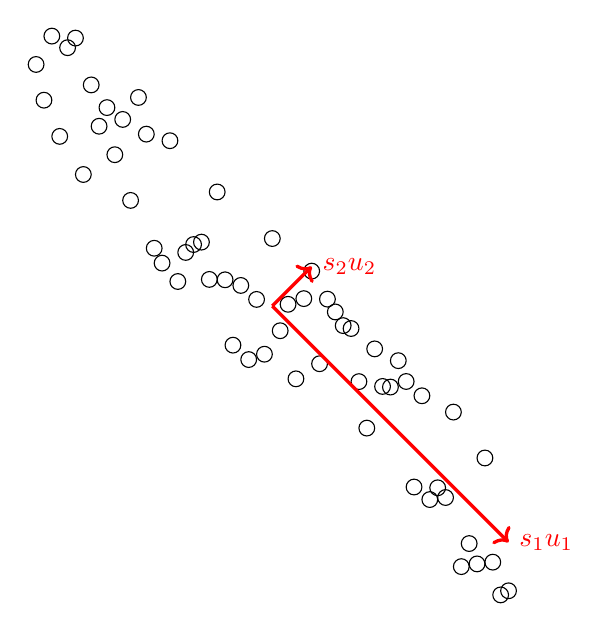
\begin{tikzpicture}

    % Draw Grid
%    \draw[<->, very thick] (-3, 0) -- (3, 0);
%    \draw[<->, very thick] (0, -3) -- (0, 3);
%    \draw[<->, very thick] (-2, -2) -- (2, 2);
    
    % Add Points
    \foreach \x in {-30, ..., 30}{
        \draw[] (-\x/10, \x/10 + rand) circle (0.1cm);
    }
    
    % Draw PCA
    \draw[very thick, red, ->] (0, 0) -- (3,-3) node[anchor=west] {$s_1 u_1$};
    \draw[very thick, red, ->] (0, 0) -- (0.5, 0.5) node[anchor=west] {$s_2 u_2$};
\end{tikzpicture}
\end{figure}






\end{document}
